\documentclass{beamer}
\usepackage{tikz}

\usetheme{default}

\title{Ramanujanovi grafi}
\author{Tadej Petrič}

\begin{document}

\begin{frame}[plain]
    \titlepage
\end{frame}

\begin{frame}
    \frametitle{Motivacija}
    Povezave računalniških naprav v omrežju
\end{frame}
\begin{frame}
    \frametitle{Motivacija}
    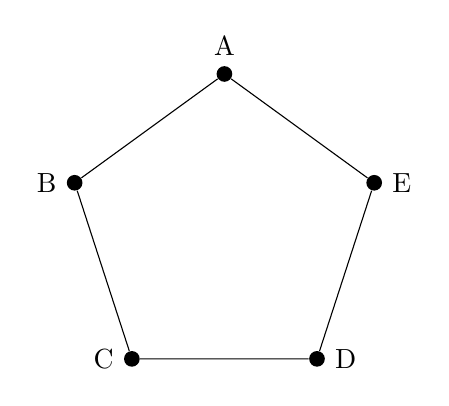
\begin{tikzpicture}
        \node[circle, fill=black, inner sep=2pt, label=above:A] (A) at (90:2) {};
        \node[circle, fill=black, inner sep=2pt, label=left:B] (B) at (162:2) {};
        \node[circle, fill=black, inner sep=2pt, label=left:C] (C) at (234:2) {};
        \node[circle, fill=black, inner sep=2pt, label=right:D] (D) at (306:2) {};
        \node[circle, fill=black, inner sep=2pt, label=right:E] (E) at (18:2) {};
        \draw (A) -- (B) -- (C) -- (D) -- (E) -- (A);
    \end{tikzpicture}
\end{frame}
\begin{frame}
    \frametitle{Motivacija}
    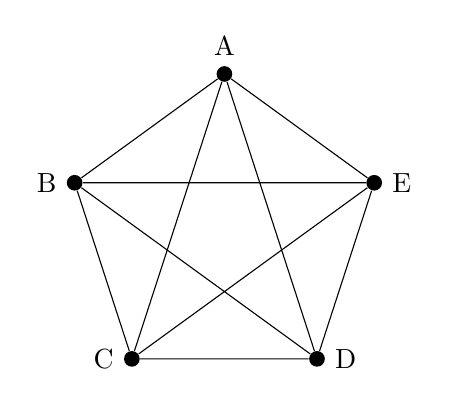
\begin{tikzpicture}
        \node[circle, fill=black, inner sep=2pt, label=above:A] (A) at (90:2) {};
        \node[circle, fill=black, inner sep=2pt, label=left:B] (B) at (162:2) {};
        \node[circle, fill=black, inner sep=2pt, label=left:C] (C) at (234:2) {};
        \node[circle, fill=black, inner sep=2pt, label=right:D] (D) at (306:2) {};
        \node[circle, fill=black, inner sep=2pt, label=right:E] (E) at (18:2) {};
        \draw (A) -- (B) -- (C) -- (D) -- (E) -- (A);
        \draw (A) -- (C) -- (E) -- (B) -- (D) -- (A);
    \end{tikzpicture}
\end{frame}
% BEGIN CHEEGER
\begin{frame}
    \frametitle{Cheegerjeva konstanta}
    Ločevanje grafa na dva dela
    \begin{itemize}
        \item \(G = (V, E)\) povezan graf
        \item \(S \subseteq V\) množica vozlišč (\(|S| \leq \frac{|V|}{2}\))
        \item \(\partial S\subseteq E\) množica povezav od \(S\) do \(\overline S\) \pause
        \item Želimo, da za velik \(|S|\) tudi velik \(\partial S\)
    \end{itemize}
    \pause
    \[
        c(G) = \min_S\frac{|\partial S|}{|S|}
    \]
\end{frame}
\begin{frame}{Primeri - Cheegerjeva konstanta}
    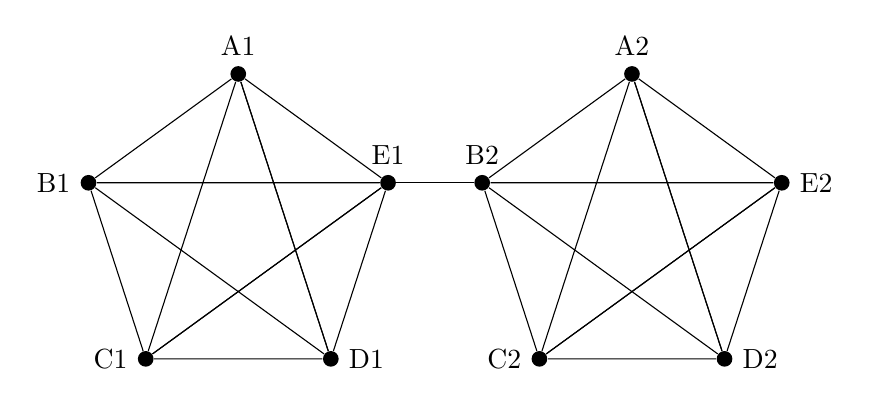
\begin{tikzpicture}
        % First K_5
        \begin{scope}[shift={(0,0)}]
            \node[circle, fill=black, inner sep=2pt, label=above:A1] (A1) at (90:2) {};
            \node[circle, fill=black, inner sep=2pt, label=left:B1] (B1) at (162:2) {};
            \node[circle, fill=black, inner sep=2pt, label=left:C1] (C1) at (234:2) {};
            \node[circle, fill=black, inner sep=2pt, label=right:D1] (D1) at (306:2) {};
            \node[circle, fill=black, inner sep=2pt, label=above:E1] (E1) at (18:2) {};
            \draw (A1) -- (B1) -- (C1) -- (D1) -- (E1) -- (A1);
            \draw (A1) -- (C1) -- (E1) -- (B1) -- (D1) -- (A1);
            \draw (A1) -- (D1);
            \draw (B1) -- (E1);
            \draw (C1) -- (E1);
        \end{scope}

        % Second K_5
        \begin{scope}[shift={(5,0)}]
            \node[circle, fill=black, inner sep=2pt, label=above:A2] (A2) at (90:2) {};
            \node[circle, fill=black, inner sep=2pt, label=above:B2] (B2) at (162:2) {};
            \node[circle, fill=black, inner sep=2pt, label=left:C2] (C2) at (234:2) {};
            \node[circle, fill=black, inner sep=2pt, label=right:D2] (D2) at (306:2) {};
            \node[circle, fill=black, inner sep=2pt, label=right:E2] (E2) at (18:2) {};
            \draw (A2) -- (B2) -- (C2) -- (D2) -- (E2) -- (A2);
            \draw (A2) -- (C2) -- (E2) -- (B2) -- (D2) -- (A2);
            \draw (A2) -- (D2);
            \draw (B2) -- (E2);
            \draw (C2) -- (E2);
        \end{scope}

        % Connecting edge between the two K_5 graphs
        \draw (E1) -- (B2);
    \end{tikzpicture}\pause
    \[c(G) = \frac{1}{5}\]
\end{frame}
\begin{frame}{Primeri - Cheegerjeva konstanta}

    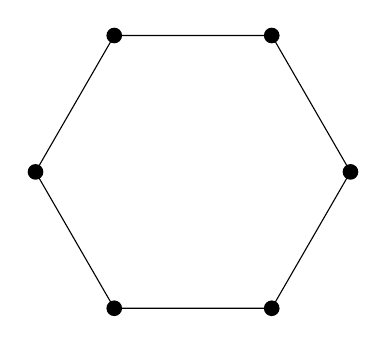
\begin{tikzpicture}
        % Defining the vertices of the cycle
        \foreach \x in {0,60,...,300} {
                \node[circle, fill=black, inner sep=2pt] at (\x:2) {};
            }
        % Drawing the edges of the cycle
        \draw (0:2) -- (60:2) -- (120:2) -- (180:2) -- (240:2) -- (300:2) -- cycle;
    \end{tikzpicture}

    \pause
    Primer za \(n\)-cikel.
    \[c(C_n) = \frac{2}{\lfloor \frac n2\rfloor}\]
\end{frame}
\begin{frame}{Primeri - Cheegerjeva konstanta}
    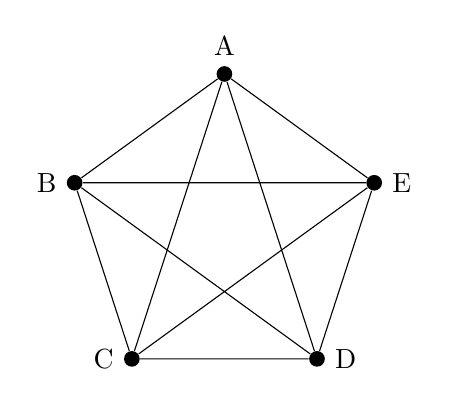
\begin{tikzpicture}
        \node[circle, fill=black, inner sep=2pt, label=above:A] (A) at (90:2) {};
        \node[circle, fill=black, inner sep=2pt, label=left:B] (B) at (162:2) {};
        \node[circle, fill=black, inner sep=2pt, label=left:C] (C) at (234:2) {};
        \node[circle, fill=black, inner sep=2pt, label=right:D] (D) at (306:2) {};
        \node[circle, fill=black, inner sep=2pt, label=right:E] (E) at (18:2) {};
        \draw (A) -- (B) -- (C) -- (D) -- (E) -- (A);
        \draw (A) -- (C) -- (E) -- (B) -- (D) -- (A);
    \end{tikzpicture}
    \pause
    Primer za \(K_n\).
    \[c(K_n) = \lceil \frac n2\rceil\]
\end{frame}
% END CHEEGER
% BEGIN SPECTRAL GAP
\begin{frame}{Spektralna luknja}
    Obstaja soroden pojem Cheegerjeve konstante - spektralna luknja.

    \(\lambda_i\) lastne vrednosti sosednostne matrike grafov.
    \[
        \lambda_1 \geq \lambda_2 \geq \ldots \geq \lambda_n
    \]

    \[
        s(G) = \lambda_1 - \lambda_2
    \]
\end{frame}
\begin{frame}{Lastne vrednosti grafov - primeri}
    \begin{itemize}
        \item \(K_n\): \((n-1, -1, \ldots, -1)\)
        \item \(K_{d,d}\): \((d,0,\ldots,0,-d)\)
              % https://chatgpt.com/c/79158977-a958-4a94-93f4-3a819352ce62
              % https://www.win.tue.nl/~aeb/2WF02/easyspectra.pdf
        \item \(C_n\): \(\left(2\cos\frac{2\pi k}{n}\right)_{k=0}^{n-1}\)
    \end{itemize}
\end{frame}
\begin{frame}{Lastne vrednosti grafov - primeri}
    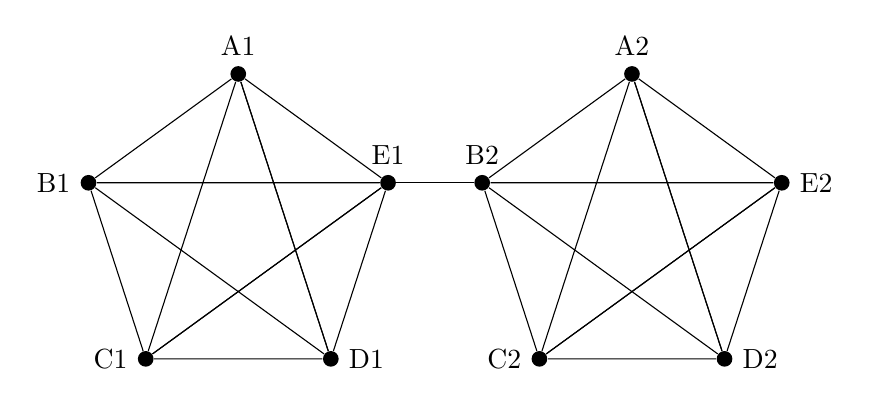
\begin{tikzpicture}
        % First K_5
        \begin{scope}[shift={(0,0)}]
            \node[circle, fill=black, inner sep=2pt, label=above:A1] (A1) at (90:2) {};
            \node[circle, fill=black, inner sep=2pt, label=left:B1] (B1) at (162:2) {};
            \node[circle, fill=black, inner sep=2pt, label=left:C1] (C1) at (234:2) {};
            \node[circle, fill=black, inner sep=2pt, label=right:D1] (D1) at (306:2) {};
            \node[circle, fill=black, inner sep=2pt, label=above:E1] (E1) at (18:2) {};
            \draw (A1) -- (B1) -- (C1) -- (D1) -- (E1) -- (A1);
            \draw (A1) -- (C1) -- (E1) -- (B1) -- (D1) -- (A1);
            \draw (A1) -- (D1);
            \draw (B1) -- (E1);
            \draw (C1) -- (E1);
        \end{scope}

        % Second K_5
        \begin{scope}[shift={(5,0)}]
            \node[circle, fill=black, inner sep=2pt, label=above:A2] (A2) at (90:2) {};
            \node[circle, fill=black, inner sep=2pt, label=above:B2] (B2) at (162:2) {};
            \node[circle, fill=black, inner sep=2pt, label=left:C2] (C2) at (234:2) {};
            \node[circle, fill=black, inner sep=2pt, label=right:D2] (D2) at (306:2) {};
            \node[circle, fill=black, inner sep=2pt, label=right:E2] (E2) at (18:2) {};
            \draw (A2) -- (B2) -- (C2) -- (D2) -- (E2) -- (A2);
            \draw (A2) -- (C2) -- (E2) -- (B2) -- (D2) -- (A2);
            \draw (A2) -- (D2);
            \draw (B2) -- (E2);
            \draw (C2) -- (E2);
        \end{scope}

        % Connecting edge between the two K_5 graphs
        \draw (E1) -- (B2);
    \end{tikzpicture}
\end{frame}
\begin{frame}{Lastne vrednosti grafov - primeri}
    \begin{align*}
        \begin{bmatrix}
            0 & 1 & 1 & 1 & 1 & 0 & 0 & 0 & 0 & 0 \\
            1 & 0 & 1 & 1 & 1 & 0 & 0 & 0 & 0 & 0 \\
            1 & 1 & 0 & 1 & 1 & 0 & 0 & 0 & 0 & 0 \\
            1 & 1 & 1 & 0 & 1 & 0 & 0 & 0 & 0 & 0 \\
            1 & 1 & 1 & 1 & 0 & 0 & 1 & 0 & 0 & 0 \\
            0 & 0 & 0 & 0 & 0 & 0 & 1 & 1 & 1 & 1 \\
            0 & 0 & 0 & 0 & 1 & 1 & 0 & 1 & 1 & 1 \\
            0 & 0 & 0 & 0 & 0 & 1 & 1 & 0 & 1 & 1 \\
            0 & 0 & 0 & 0 & 0 & 1 & 1 & 1 & 0 & 1 \\
            0 & 0 & 0 & 0 & 0 & 1 & 1 & 1 & 1 & 0
        \end{bmatrix}
    \end{align*}
    \((\lambda_i)_1^{10} \approx (-1.83, -1, -1, -1, -1, -1, -1, -0.24, 3.83, 4.24)\)
\end{frame}
\begin{frame}{Cheegerjeva neenakost}
    Za \(d\)-regularen graf velja
    \begin{align*}
        \frac{1}{2}s(G)\leq c(G) \leq \sqrt{2d s(G)} \\
        2c(G) \geq s(G) \geq \frac{c^2(G)}{2d}
    \end{align*}
    Torej večja kot je spektralna luknja, večja je Cheegerjeva konstanta.
\end{frame}
\begin{frame}{Cheegerjeva neenakost - primeri}
    \(K_n\) za sodi \(n\): \(c(K_n) = \frac{n}{2}\), \(s(K_n) = n\)
    \[
        \frac{n}{2} \leq \frac{n}{2} \leq \sqrt{2n(n-1)}
    \]
    \(C_n\) za sodi \(n\): \(c(C_n) = \frac{4}{n}\), \(s(C_n) = 2\left(1-\cos\left(\frac{2\pi}{n}\right)\right)\)
    \[
        1-\cos\left(\frac{2\pi}{n}\right) \leq \frac{4}{n} \leq 2\sqrt{2\left(1-\cos\left(\frac{2\pi}{n}\right)\right)}
    \]
    % https://www.desmos.com/calculator/4yx13carzp
\end{frame}
% END SPECTRAL GAP
% BEGIN RAMANUJAN
\begin{frame}
    \frametitle{Alon-Boppanov izrek}
    Imamo družino \(G_n\) d-regularnih grafov. \(\lambda_i\) druga največja lastna vrednost. \(|G_n| \to \infty\)
    \begin{align*}
        \lambda_i \geq 2\sqrt{d-1} -o_n(1) \\
    \end{align*}
    Oziroma
    %https://www.math.mcgill.ca/goren/667.2010/Luiz.pdf
    \begin{align*}
        \liminf_{i\to\infty} \lambda_i \geq 2\sqrt{d-1}
    \end{align*}
    Manjša kot je \(\lambda_i\), večja je \(s(G_i)\)!
\end{frame}
\begin{frame}
    \frametitle{Ramanujanovi grafi}
    Optimalni grafi glede na Alon-Boppanov izrek. \pause

    So d-regularni grafi za katere velja
    \[
        \lambda \leq 2\sqrt{d-1}
    \]
    oziroma
    \[
        s(G) \geq d-2\sqrt{d-1}
    \]
\end{frame}
\begin{frame}
    \frametitle{Ramanujanovi grafi - primeri}
    \(K_n\) za sodi \(n\): \(s(K_n) = n\)
    \begin{itemize}
        \item \(n \geq n-2\sqrt{n-2}\)
    \end{itemize}
    Je Ramanujanov graf.

    Vsi 2-regularni grafi so Ramanujanovi.
\end{frame}
\begin{frame}
    \frametitle{Ramanujanovi grafi - protiprimer}
    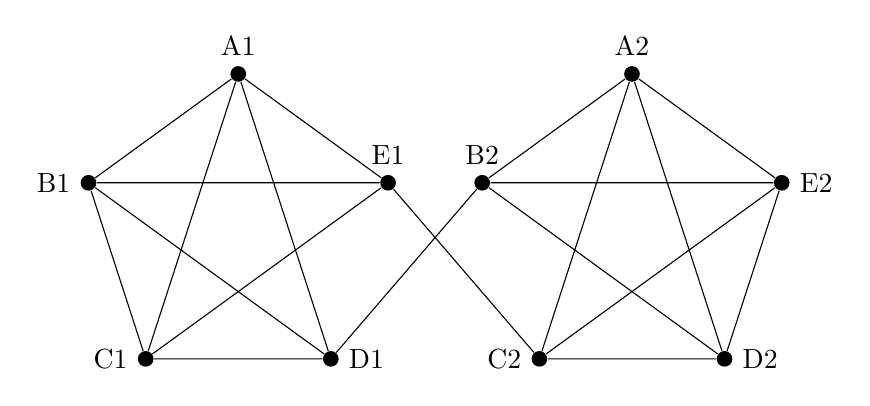
\begin{tikzpicture}
        % First K_5
        \begin{scope}[shift={(0,0)}]
            \node[circle, fill=black, inner sep=2pt, label=above:A1] (A1) at (90:2) {};
            \node[circle, fill=black, inner sep=2pt, label=left:B1] (B1) at (162:2) {};
            \node[circle, fill=black, inner sep=2pt, label=left:C1] (C1) at (234:2) {};
            \node[circle, fill=black, inner sep=2pt, label=right:D1] (D1) at (306:2) {};
            \node[circle, fill=black, inner sep=2pt, label=above:E1] (E1) at (18:2) {};
            \draw (A1) -- (B1) -- (C1) -- (D1);
            \draw (E1) -- (A1);
            \draw (A1) -- (C1) -- (E1) -- (B1) -- (D1) -- (A1);
        \end{scope}

        % Second K_5
        \begin{scope}[shift={(5,0)}]
            \node[circle, fill=black, inner sep=2pt, label=above:A2] (A2) at (90:2) {};
            \node[circle, fill=black, inner sep=2pt, label=above:B2] (B2) at (162:2) {};
            \node[circle, fill=black, inner sep=2pt, label=left:C2] (C2) at (234:2) {};
            \node[circle, fill=black, inner sep=2pt, label=right:D2] (D2) at (306:2) {};
            \node[circle, fill=black, inner sep=2pt, label=right:E2] (E2) at (18:2) {};
            \draw (A2) -- (B2);
            \draw (C2) -- (D2) -- (E2) -- (A2);
            \draw (A2) -- (C2) -- (E2) -- (B2) -- (D2) -- (A2);
        \end{scope}

        % Connecting edge between the two K_5 graphs
        \draw (E1) -- (C2);
        \draw (D1) -- (B2);
    \end{tikzpicture}
    \pause
    \[
        \lambda \approx 3.55 > 2\sqrt{4-1} \approx 3.46
    \]
    \pause
    Velja za vse združke od (vključno) \(K_5\) naprej.
\end{frame}
% END RAMANUJAN
% BEGIN KONSTRUKCIJE
\begin{frame}{Caylejevi grafi \(\mathbb Z_4\)}
    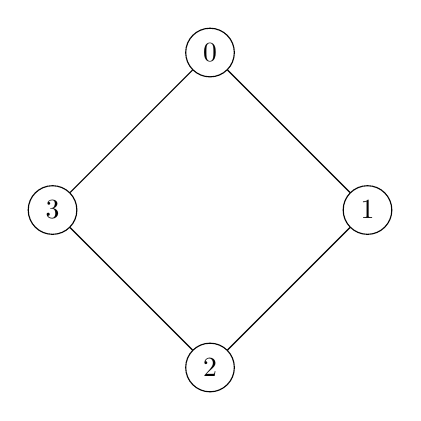
\begin{tikzpicture}
        % Define the style for the nodes
        \tikzset{every node/.style={draw,circle}}

        % Nodes
        \node (1) at (0,2) {0};
        \node (2) at (2,0) {1};
        \node (3) at (0,-2) {2};
        \node (4) at (-2,0) {3};

        % Edges
        \draw (1) -- (2);
        \draw (2) -- (3);
        \draw (3) -- (4);
        \draw (4) -- (1);
    \end{tikzpicture}
\end{frame}

\end{document}

np.array([[0, 1, 1, 1, 1, 0, 0, 0, 0, 0],
        [1, 0, 1, 1, 1, 0, 0, 0, 0, 0],
        [1, 1, 0, 1, 1, 0, 0, 0, 0, 0],
        [1, 1, 1, 0, 0, 0, 1, 0, 0, 0],
        [1, 1, 1, 1, 0, 0, 0, 1, 0, 0],
        [0, 0, 0, 0, 0, 0, 1, 1, 1, 1],
        [0, 0, 0, 1, 0, 1, 0, 1, 1, 1],
        [0, 0, 0, 0, 1, 1, 1, 0, 1, 1],
        [0, 0, 0, 0, 0, 1, 1, 1, 0, 1],
        [0, 0, 0, 0, 0, 1, 1, 1, 1, 0]])